\section{去信任的清算协议}\label{sec:clearing}

本节先介绍去信任清算的基本概念,帮助读者比较直观的理解闪电网络的思想和理念,想了解更多源代码的读者看完这一节后,请参考附录 \ref{sec:codes}。

\subsection{基本概念}

\subsubsection{虚拟银行 Virtual Bank}
虚拟银行是运行于区块链上的一个智能合约,由支付双方共同协商创建。它模拟一个银行机构作为支付双方的公共债务人。虚拟银行部署之后,按照预先协商的额度,双方向虚拟银行的智能合约注入资金,完成虚拟银行的筹建。如果虚拟银行被清盘结算,资金都返还给支付双方,那么虚拟银行的服务自行终结。

\begin{figure}[h!]
    \centering
    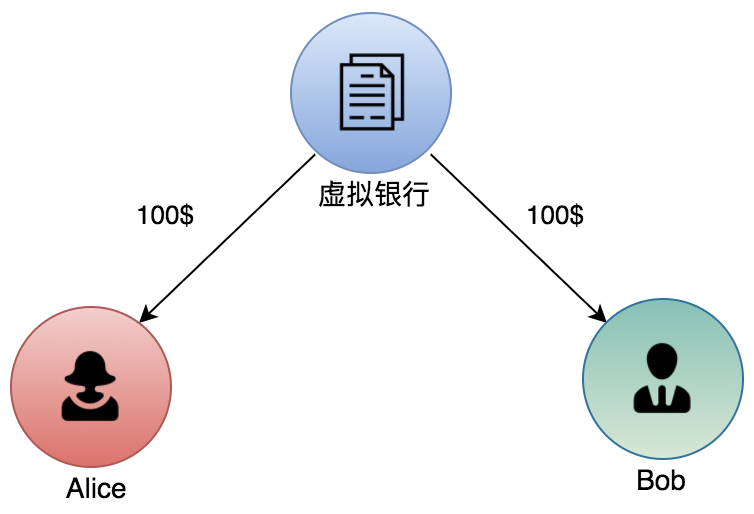
\includegraphics[width=8cm, keepaspectratio]{../images/channel.png}
    \caption{虚拟银行}
    \label{fig:virtualbank}
\end{figure}

和传统的银行相比,虚拟银行有四个特点:

\begin{itemize}
    \item \textbf{微型}: 一个虚拟银行只有两个账户,所以资产负债表也只有2条数据。
    \item \textbf{无需信任}:虚拟银行是通过智能合约实现的,继承了智能合约的公开、透明、不可篡改、不可伪造、不可撤销等特点。所以作为公共债务人,虚拟银行没有传统金融机构的风险:比如对手风险、道德风险、流动性风险等。虚拟银行筹建完成之后,它的债务偿付能力永远是100\%,自然也不没有金融监管的成本。提供了无需信任的资产托管服务。
    \item \textbf{用户自治}: 虚拟银行只是一个智能合约,并不是一个独立的运营机构。所以银行的资产管理由两个用户共同协商管理。
    \item \textbf{双重签名}:银行只有两个账户,而且总资产不变。一方的资产增加,意味着另一方的资产减少,这是一个零和博弈。为了防止单方面作弊行为,侵害对方的权益,虚拟银行智能合约在处理资产调整请求的时候,要验证双方的签名,保证每一次资产调整都是双方共同的真实意愿。
\end{itemize}


\subsubsection{共同承诺 (Mutual Commitment)} \label{sec:commiment}
每一次微支付,虚拟银行中的资产负债表要做一次调整。双方在链下对债务调整方案达成一致,形成向虚拟银行智能合约的请求消息,并且双方签名。此消息并不立刻广播到链上,而是由双方存储在本地,称之为\textbf{共同承诺}。共同承诺是双方真实意愿的表达,是彼此之间对资产分配方案的承诺。共同承诺一旦达成,在任何时候、任何一方都可以将承诺方案广播到链上,虚拟银行都会按照承诺方案结算银行的资产。共同承诺的作用类似于银行支票,虽然没有兑现,但是持有共同承诺就可以无风险的、随时的从虚拟银行中兑现响应的资产。

共同承诺的实现必须满足以下几个要求:

\begin{enumerate}
    \item \textbf{不可伪造}:共同承诺表达虚拟银行双方当事人的真实意愿,任何第三方无法伪造当事人的身份,生成虚假共同承诺。
    \item \textbf{不可篡改}:对于已经达成的承诺,其中的所有条款无法篡改。虚拟银行智能合约会检查双方的签名,确保承诺的完整性。
    \item \textbf{可以覆盖}:只要虚拟银行还没有兑现共同承诺,就可以被新的承诺覆盖。对于交易双方来讲,只有最后的一份共同承诺是有效的,之前被覆盖的历史承诺都相当于已经被撤销。共同承诺在技术上有撤销机制。
    \item \textbf{文义证券}:在共同承诺的条款限定条件下,虚拟银行必须能够随时的、无风险的、按照承诺约定的分配方案结算资产。或者说,共同承诺具有文义证券、无因证券的特点。
\end{enumerate}

通俗的来讲,共同承诺就像是双方共同签署的银行支票,虚拟银行可以在任何时候兑现这张支票。和常规意义的支票不同的:它同时处置两个人的全部资产,一旦兑现某一个承诺,虚拟银行所有资产被清算,随即关闭。

闪电网络协议中有两种承诺方案:RSMC 承诺与 HTLC 承诺。他们的区别我们后面会讲,但是都满足上述4个条件。

\subsubsection{承诺编号 Sequence}
在共同承诺兑现之前,双方可以达成多次共同承诺,撤销旧的承诺,建立新的承诺。这些承诺按照时间顺序编号,以 Sequence 表示。

需要注意的是,闪电网络白皮书中的 Sequence 和本文的定义是不一样的。原文里的 Sequence 是一种时间锁,本文里只是一个简单的编号。但是二者的设计目的都是实现承诺方案的可以撤销机制。所以读者可以暂时忽略二者的技术差异。


\subsubsection{进攻方(Attacker) 与 防御方(Defender)}
如果一方将共同承诺广播到链上,主动向虚拟银行发起申请, 重新结算资产,此方称之为承诺方案的进攻方。被动的接受对方资产分配方案的一方,称之为防御方。

虚拟银行的资产清算,相当于瓜分银行的总资产,是一种零和博弈。假设双方都是理性的决策者,任何一方都不会做出于对方有利,于己方不利的决策。双方需要一种公平的机制管理共同承诺,规避对手风险,防止对方作弊。

在闪电网络的协议里,一个新的承诺方案先由防御方初审。如果防御方接受此承诺方案,就对此方案签名,然后发送给进攻方进行二审。
进攻方持有多个防御方已初审的承诺方案,有权放弃对己方不利的方案。
同时有权选择广播共同承诺的时间,当他觉得合适的时候,再加上自己的签名,广播到链上,向虚拟银行请求结算资产。
虚拟银行智能合约检验双方的签名,根据共同承诺的条款,公开、透明的结算双方的资产。

\subsubsection{对偶承诺方案 Dual Commitment}
和现实中的支票不同,共同承诺都是一式两份,双方各持有一份。两份承诺编号一致、分配方案一致。
但是攻守位置互换。比如说 Alice 持有的那一份,Alice 是进攻方,Bob 是防御方(Bob已经初审签名);
反之,Bob 持有的那一份中,Bob 是进攻方,Alice 是防御方(Alice 已经初审签名)。
这两份承诺方案是一对,互为对偶承诺方案,具有同等效力。
虚拟银行可以接受任何一份,但是只能接受一份。
一份承诺被兑现,另外一份立即作废。

这样设计的好处有两个:一是保持共同承诺的活性,避免单点故障造成的死锁。
因为防御方只能被动等待进攻方向虚拟银行发起请求。
假如进攻方故障,不能行使进攻方的职责,防御方可以翻转角色,使用对偶承诺方案,以进攻方的身份完成资产的结算。
二是保持灵活性和对称性,任何一方都可以随时主动兑现共同承诺,降低对手风险。

\subsubsection{撤销锁 Revocation Lock}
为了标识一个共同承诺方案已经被覆盖,闪电网络协议设计了撤销锁机制。
在每一份承诺方案中,进攻方必须要放置一个撤销锁。
不同的承诺编号、不同的承诺方案镜像有不同的撤销锁。
如果一共有 $N$ 对承诺方案,那么需要有 $2N$ 个不同的撤销锁。

撤销锁由承诺方案的进攻方管理,它实际是一个随机账户地址,对应的私钥由进攻方创建。
如果进攻方要撤销某一个承诺方案,他必须公开对应的撤销锁私钥。
反过来说,如果防御方从进攻方拿到了一个撤销锁的私钥,那么他可以相信进攻方确实放弃了对应的承诺方案。 

一般来讲,从虚拟银行开始,一共有 $N$ 对共同承诺方案,前面的 $(N - 1)$ 对承诺方案已经被覆盖。
这些历史承诺方案的撤销锁私钥是公开的,每一方都会保留一份对方的\textbf{撤销锁私钥列表}。
只有最后一对承诺方案是有效的,其撤销私钥还没有公开。

撤销锁的安全机制:当一个承诺方案提交给虚拟银行的时候,防御方可以查看此撤销锁的编号(Sequence)。
如果防御方发现此承诺方案是已经被覆盖的,那么从\textbf{撤销锁私钥列表}中,找到对应的私钥,并且生成签名作为凭证,向虚拟银行证明对应的承诺方案是已经被覆盖的。
虚拟银行将判定进攻方违约,对进攻方处以罚金。
这种情况称之为“\textbf{破解撤销锁}”。
所以如果进攻方是理性的,他就不会冒着撤销锁被破解的风险提交已经覆盖的承诺方案。
反之,提交未被覆盖的承诺方案是安全的,因为防御方不知道撤销锁私钥,也就无法破解撤销锁。

当双方创建一对新的承诺方案的时候,需要交换旧承诺方案的失效私钥,表示双方都只承认新的方案,覆盖旧的方案。
在承诺方案兑现之前,双方都要妥善保存对方的\textbf{撤销锁私钥列表},防止对方使用对己方不利的承诺提案结算虚拟银行中的资产。

\subsubsection{诚信保证金 Fidelity Bond}
为了保证承诺方案的公平性,承诺方案会设立\textbf{诚信保证金}条款,和撤销锁机制配合使用。
当虚拟银行兑现一份承诺方案的时候,防御方被动接受进攻方的资产分配方案,所以防御方的资产份额可以优先结算。
而进攻方的所有资产作为\textbf{诚信保证金}冻结一段时间。
目的是防止进攻方提交一份已经被覆盖的承诺方案,侵犯防御方的利益。这个时间段成为\textbf{冻结期 Freeze Time}

在\textbf{诚信保证金}的冻结期间内,虚拟银行会等待防御方破解该方案的撤销锁。
如果破解成功,防御方可以取走所有的诚信保证金作为惩罚,进攻方就会损失所有资产。
反之,冻结期满之后,进攻方可以取走诚信保证金。

\subsubsection{支付通道}
支付双方以虚拟银行托管双方的资产,通过共同承诺重新清算双方的存款余额,以达到价值转移的效果,这种支付工具称之为支付通道。
虚拟银行筹建并且达成初始共同承诺,标志着支付通道的开启;
虚拟银行根据任何一方提交的承诺方案结算双方的资产,就标志着支付通道关闭。

\subsection{RSMC承诺方案}
\subsubsection{RSMC承诺方案的数据结构}
在闪电网络中定义了两种承诺方案。第一种称为 RSMC(Recoverable Sequence Maturity Contract)承诺方案。
本文中,一个 RSMC 使用如图 \ref{fig:rsmc} 的图形化表示,它包含了承诺方案的最基本元素。
其中包括承诺编号、撤销锁、诚信保证金、对偶承诺方案等。

\begin{figure}[h!]
    \centering
    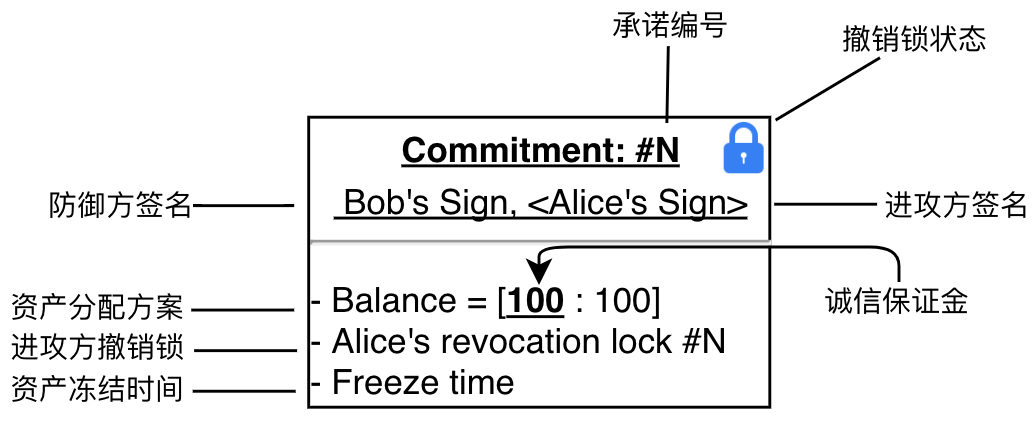
\includegraphics[width=12cm, keepaspectratio]{../images/RSMC.png}
    \caption{RSMC 承诺方案的数据结构}
    \label{fig:rsmc}
\end{figure}

RSMC承诺方案分为 Header 与 Body 两部分。
\begin{itemize}
    \item Header 部分的数据有
        \begin{enumerate}
            \item \textbf{承诺编号}:此例中为 \#$N$。如 所述,每一个编号的承诺都是一式两份,分别为 Alice 和 Bob 持有。这两份承诺互为对偶承诺,攻守位置互换。左面Alice 持有的承诺是以 Alice 为进攻方,Bob 为防御方;反之,右面 Bob 持有的承诺以 Bob 为进攻方,Alice 为防御方。
            \item \textbf{双方的签名}:防御方作为初审,已经在承诺里面签名。进攻方的签名暂时还空着。比如说左面 Alice 的承诺中有 Bob 的签名"Bob's Sign",Alice 还未签名,用"<Alice's Sign>"表示。
            \item \textbf{撤销锁状态}: 表示撤销锁对应的私钥已经公开,本承诺方案已经被覆盖。
        \end{enumerate}
        
    \item Body 部分的数据有
        \begin{enumerate}
            \item \textbf{资产分配方案}:双方约定如何分配虚拟银行的资产,因为这一第一份方案,所以和双方的注资额度是一样的,也是[100, 100]。
            \item \textbf{诚信保证金}: 资产分配方案中,进攻方一方的资产(下划线标识)作为诚信保证金将会被锁定一段时间。
            \item \textbf{进攻方的撤销锁}: 由进攻方设定的撤销锁,对应的私钥由进攻方管理。如果此方案撤销,进攻方要公开撤销锁的私钥。
            \item \textbf{资产冻结时间}:诚信保证金的冻结时间。此时间要足够长,使得防御方有足够的时间审查进攻方提交的承诺方案。
        \end{enumerate}
\end{itemize}

\subsubsection{通过 RSMC 承诺方案进行支付}

假设 Alice 和 Bob 创建了一个虚拟银行,上方初始的资产为 [100, 100]。
双方的第一份共同承诺的方案如图 \ref{fig:rsmc_1} 所示。
这份初始承诺方案按照[100, 100] 的方式分配银行资产。承诺方案的的编号为 $\#1$,一式两份。
左侧的一份以 Alice 为进攻方,右侧的一份以 Bob 为进攻方。这两份互为对偶承诺。
\begin{figure}[h!]
    \centering
    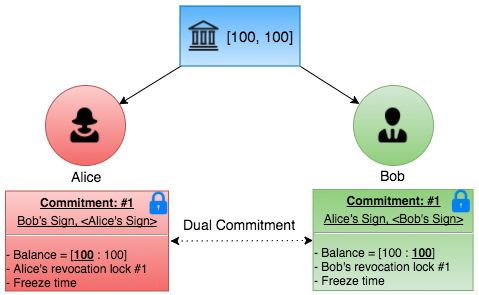
\includegraphics[width=8cm, keepaspectratio]{../images/rsmc_1.png}
    \caption{初始的 RSMC 承诺方案}
    \label{fig:rsmc_1}
\end{figure}

如果 Alice 向 Bob 支付 10 美元,双方会创建一个新的 RSMC 承诺方案,编号为 $\#2$。
分配方案改为:[90, 110]。如下图 \ref{fig:rsmc_2} 所示。
我了覆盖旧承诺方案,双方互相公开编号为 $\#1$ 的承诺方案的撤销锁私钥。
同时注意在新的承诺方案里必须使用新的撤销锁。

\begin{figure}[h!]
    \centering
    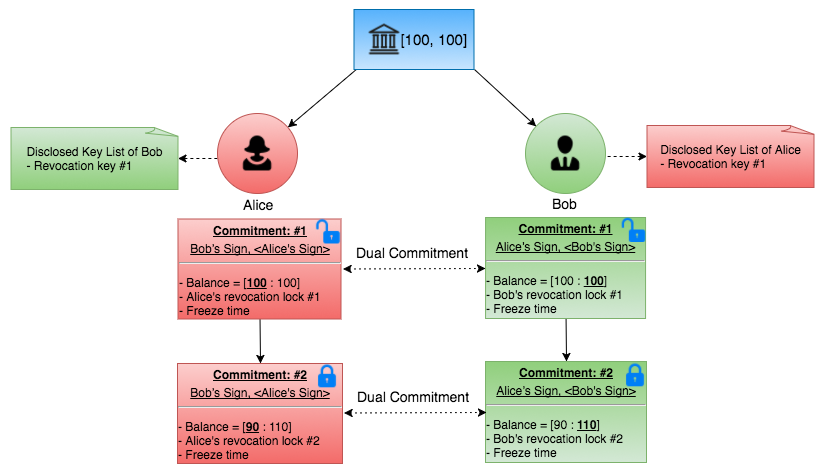
\includegraphics[width=16cm, keepaspectratio]{../images/rsmc_2.png}
    \caption{更新 RSMC 承诺方案}
    \label{fig:rsmc_2}
\end{figure}

RSMC 承诺方案的特点是没有时间期限,只要没有被撤销,承诺永久有效。
任何一方随时可以向虚拟银行提交 RSMC 承诺方案。

\subsubsection{RSMC 承诺方案的对手风险问题}
在图 \ref{fig:rsmc_2} 的支付过程中,对于 Alice 来讲,使用新的 RSMC 承诺覆盖旧的承诺方案会损失 10 美元。
所以她不会无缘无故的公开编号为 $\#1$ 的承诺方案的撤销锁私钥。
这种情况下,需要外部的支付环境保证支付的达成。
比如说,Alice 向 Bob 购买 10 美元的商品,这时候 Alice 会自愿的撤销旧承诺。

\subsection{HTLC 承诺方案}\label{sec:htlc}
\subsubsection{支付路径}
RSMC 协议的局限性在于虚拟银行自有两个账户,只能服务于两个人之间的往来支付。
支付双方必须建立直连的支付通道。
如果在 $N$ 个人之间建立支付通道,那么每个人需要管理 $(N-1)$ 个支付通道,总计一共有 $(N - 1)*N/2$  个支付通道。
闪电网络进一步提出了支付路径的概念,可以将支付通道的复杂度从 $O(N^2)$ 降低到 $O(N)$。

如图 \ref{fig:alice_bob_carol} 所示,Alice 和 Carol 之间没有建立支付通道。
但是 Alice 和 Bob,以及 Bob 和 Carol 之间建立了支付通道。这两条支付通道首尾相连,链接成了一个最简单的支付路径。
如果 Alice 向 Carol 支付 10 美元,那么可以通过这条支付路径完成。

\begin{figure}[h!]
    \centering
    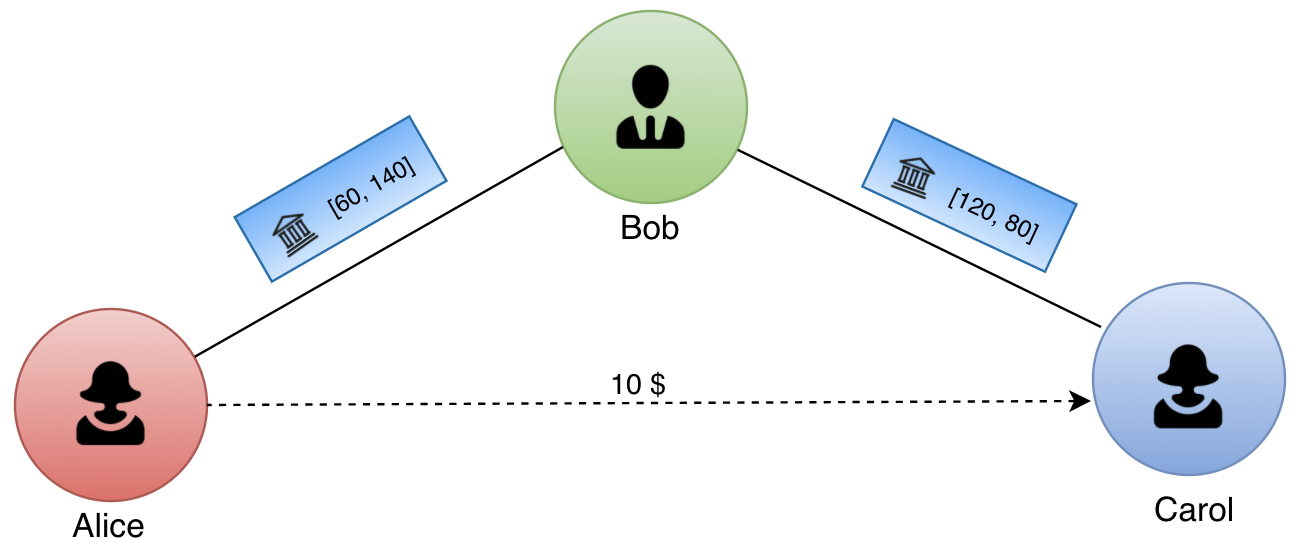
\includegraphics[width=10cm, keepaspectratio]{../images/channels_1.png}
    \caption{最简单的支付路径}
    \label{fig:alice_bob_carol}
\end{figure}

具体的来讲,就是在 Alice 和 Bob 的支付通道中,将资产分配方式从 [60, 140] 改成 [50, 150]。
同时 在 Bob 和 Carol 的支付通道中,将资产分配方式从 [120, 80] 改成 [110, 90]。
这等价于 Bob 作为中间人帮助 Alice 将 10 美元转到 Carol 手中。

支付路径可以是任意的长度,只要是联通的即可。

\subsubsection{HTLC承诺方案的数据结构}
在支付路径中,所有的支付通道是互相独立,需要一种机制保证他们的支付具有原子性:要么都完成支付,要么都没有完成支付。
为此,闪电网络提出了 HTLC (Hash Time Lock Contract) 承诺方案。
和 RSMC 一样,HTLC 中的承诺方案同样也具有不可伪造性、不可篡改性、可覆盖性、文义证券性。

如图 \ref{fig:htlc} 所示,这是一个 HTLC 承诺方案的示例。

\begin{figure}[h!]
    \centering
    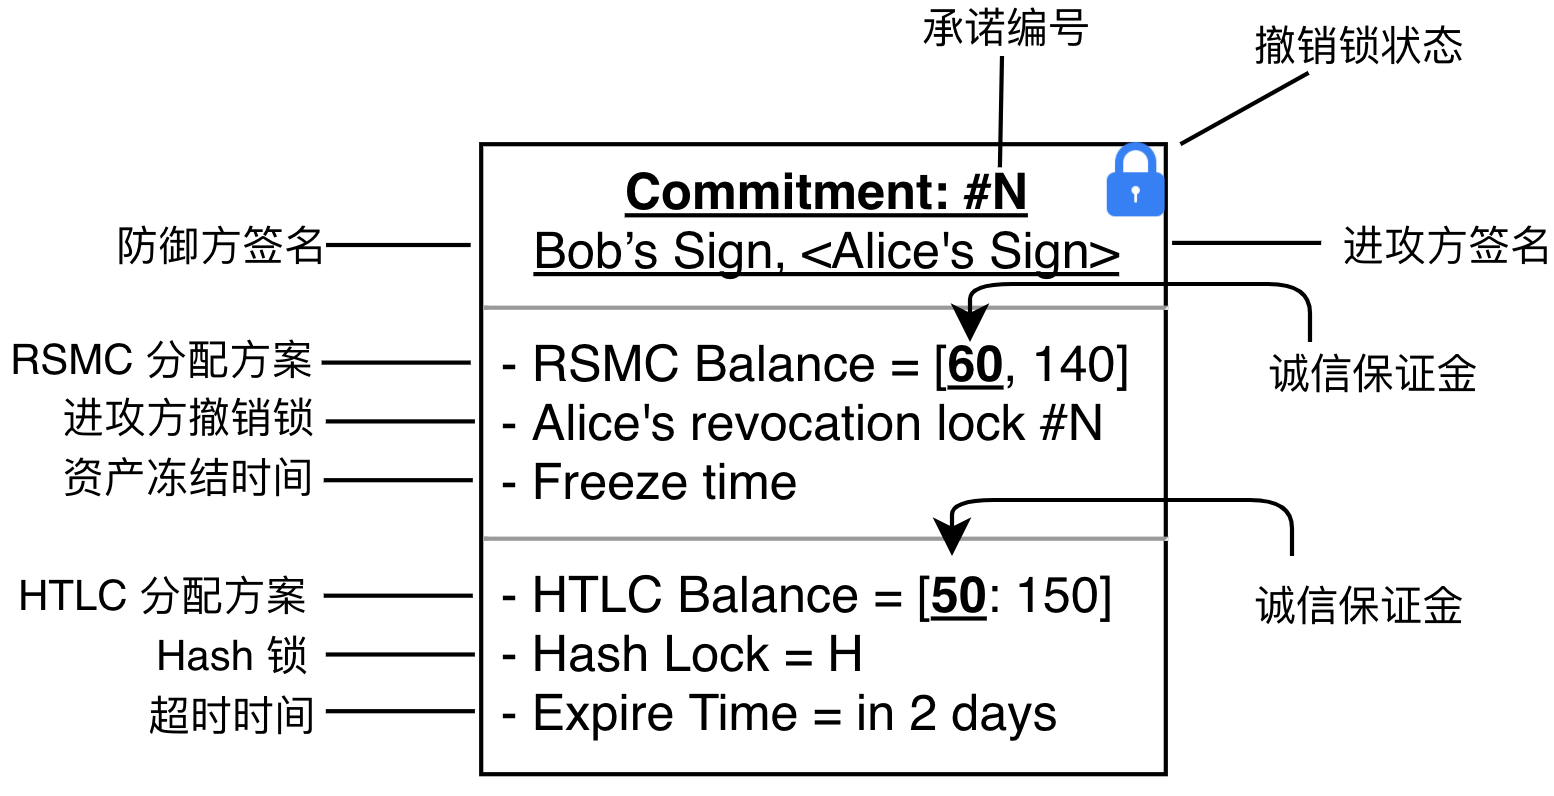
\includegraphics[width=12cm, keepaspectratio]{../images/HTLC.png}
    \caption{HTLC 承诺方案的数据结构}
    \label{fig:htlc}
\end{figure}

HTLC 承诺方案也是分为 Header 和 Body 两部分,其中 Header 部分和 RSMC 是一样的。
只是在 Body 部分有差异,它在 RSMC的 Body 部分基础上增加了 HTLC 专有条款:
\begin{itemize}
    \item HTLC 条款
        \begin{enumerate}
            \item \textbf{HTLC 资产分配方案}: 如果满足 Hash 锁与时间锁两个条件,那么就按照此方案分配资产。
            \item \textbf{Hash锁}:支付的发送方向接收方出示一个 Hash 值 H,接收方必须公开对应的暗语R,使得 Hash( R ) = H。满足此条件 HTLC 分配方案才有效。
            \item \textbf{超时时间}:HTLC 分配方案只能在超时时间内有效。
        \end{enumerate}
\end{itemize}

从语义上讲,HTLC 承诺提供两个不同的资产分配方案。如果满足下面的 Hash 锁和超时时间两个条件,那么 HTLC 分配方案生效。
反之,上面的 RSMC 分配方案生效。
换句话说,HTLC 部分是一个有条件的、短期有效的分配方案,但是优先级比上面的 RSMC 部分要高。


举个例子,假设根据当前的共同承诺编号为 $\#N$,余额是 [90, 110]。
Alice 向 Bob 支付10美元。
但是前提是 Bob 必须要在 2小时之内公开暗语 $R$,使得 $H = hash(R)$。
那么 HTLC 承诺方案的条款应该是如下图 \ref{fig:htlc_sample} 所示:

\begin{figure}[h!]
    \centering
    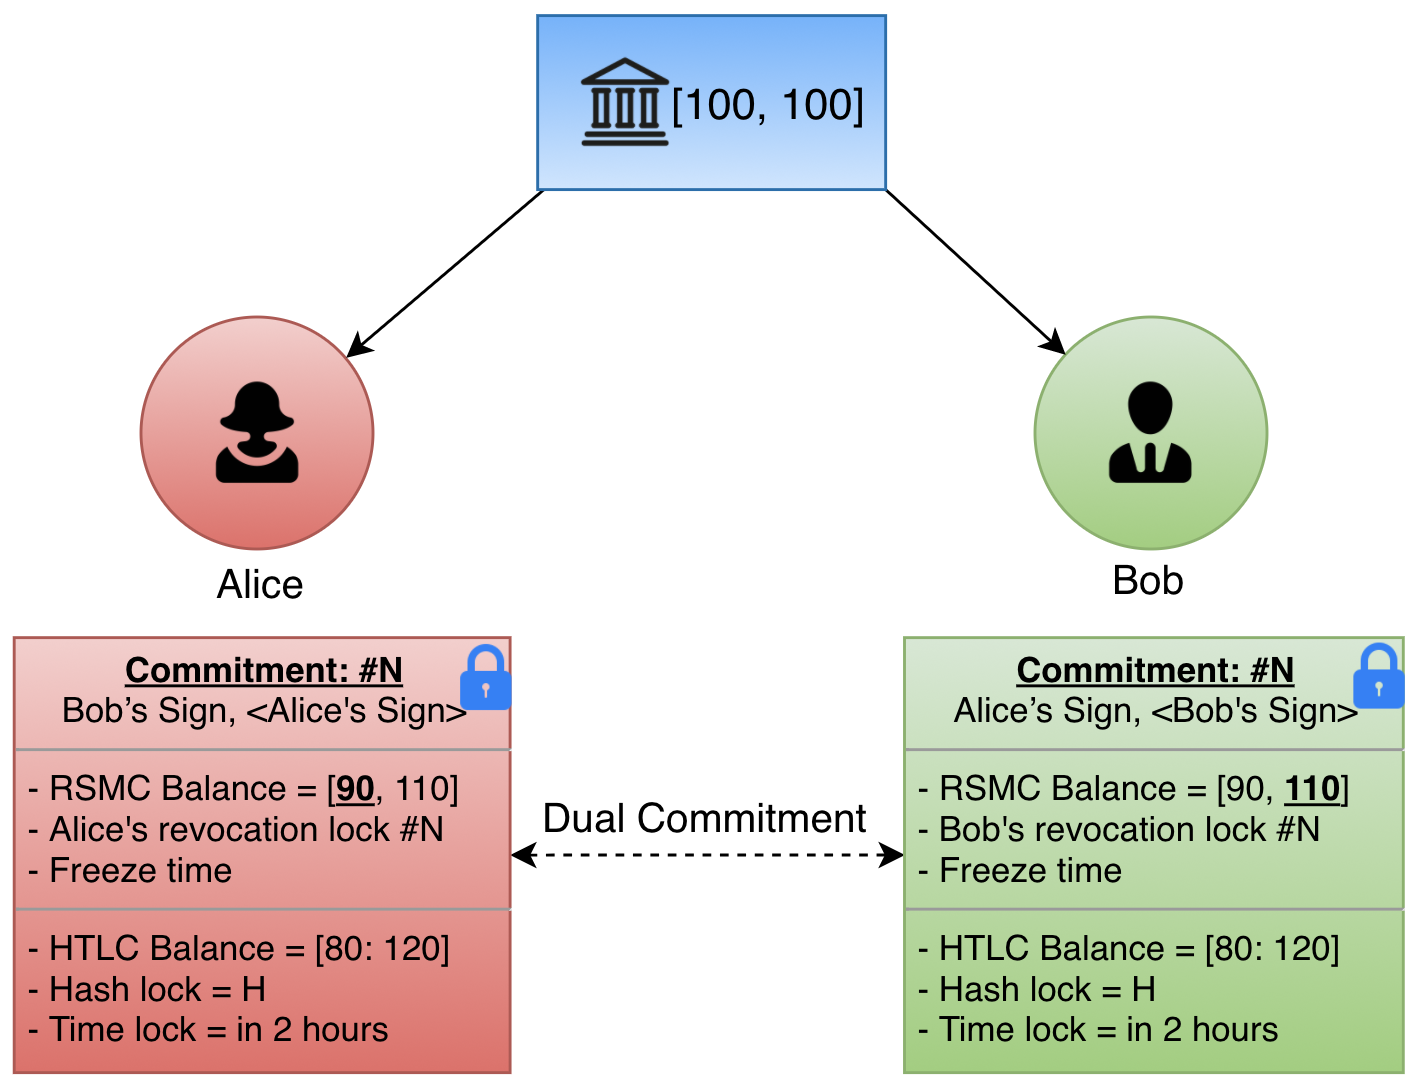
\includegraphics[width=10cm, keepaspectratio]{../images/htlc_sample.png}
    \caption{HTLC 承诺方案}
    \label{fig:htlc_sample}
\end{figure}

这一对 HTLC 承诺方案可以解读为:

\begin{itemize}
    \item 如果虚拟银行在2个小时之内接收到此承诺方案,同时提交的暗语 $R$ 满足 $H = hash(R)$ ,就按照[80,120]的方案结算 Alice 和 Bob 的资产。这相当于 Alice 向 Bob 支付了 10 美元。
    \item 如果虚拟银行再2个小时之后接收到此承诺方案,那么按照[90, 110]的方案结算 Alice 和 Bob 的资产。这相当于保持原状。
    \item 其它情况下,不做任何处理。
\end{itemize}


\subsubsection{在支付路径上使用 HTLC 进行支付} \label{sec:htlc_pay}
下面以图 \ref{fig:alice_bob_carol} 为例,介绍在支付路径上如何使用 HTLC 承诺方案完成支付。
在支付开始之前,假设 Alice-Bob 的支付通道当前承诺编号为 $N$,如图 \ref{fig:htlc_alice_bob_1} 所示。
假设 Bob-Carol 的支付通道当前承诺编号为 $M$,如图 \ref{fig:htlc_bob_carol_1} 所示。

\begin{figure}[h!]
    \centering
    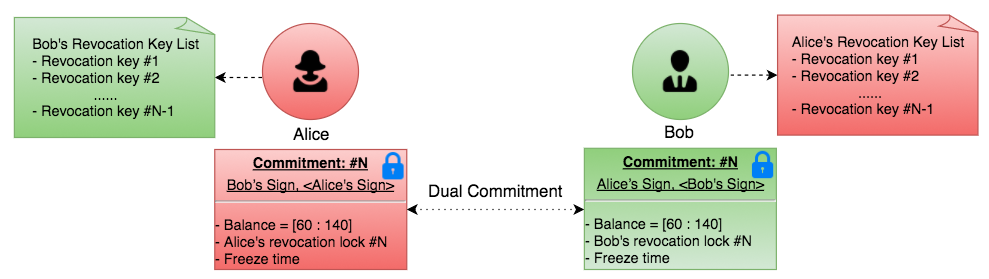
\includegraphics[width=12cm, keepaspectratio]{../images/alice_bob_1.png}
    \caption{Alice-Bob 的初始状态}
    \label{fig:htlc_alice_bob_1}
\end{figure}

\begin{figure}[h!]
    \centering
    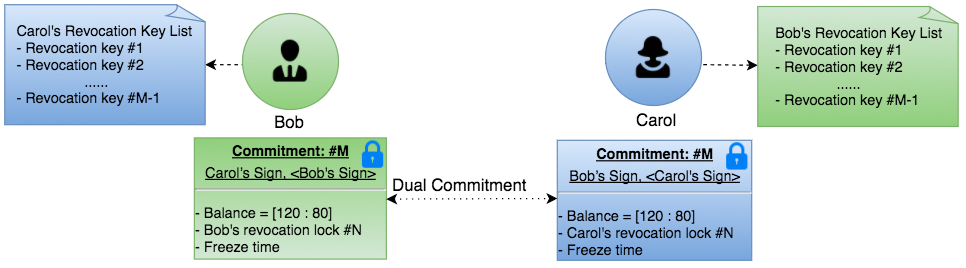
\includegraphics[width=12cm, keepaspectratio]{../images/bob_carol_1.png}
    \caption{Bob-Carol 的初始状态}
    \label{fig:htlc_bob_carol_1}
\end{figure}

\newpage
整个过程分为五步,如图 \ref{fig:htlc_path} 所示。

\begin{figure}[h!]
    \centering
    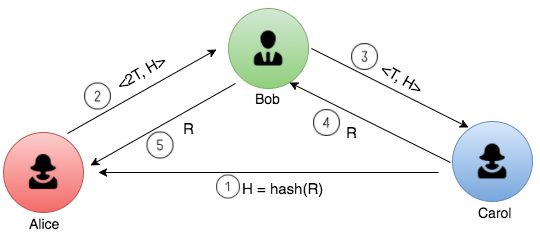
\includegraphics[width=10cm, keepaspectratio]{../images/payment_path.png}
    \caption{支付路径}
    \label{fig:htlc_path}
\end{figure}


\begin{enumerate}
    \item Carol 随机产生暗语 R,计算Hash 值: H = hash(R),并将 H 发送给 Alice。

    \item 如图 \ref{fig:htlc_alice_bob_2}, Alice 和 Bob 达成编号为 $\#(N+1)$ 的 HTLC 承诺:如果Bob能在时间 \textbf{2小时} 内出示暗语 R,使得 hash(R) = H, 那么Alice 向 Bob 支付 10 美元。同时覆盖 $\#(N)$ 的承诺方案。 
        \begin{figure}[h!]
            \centering
            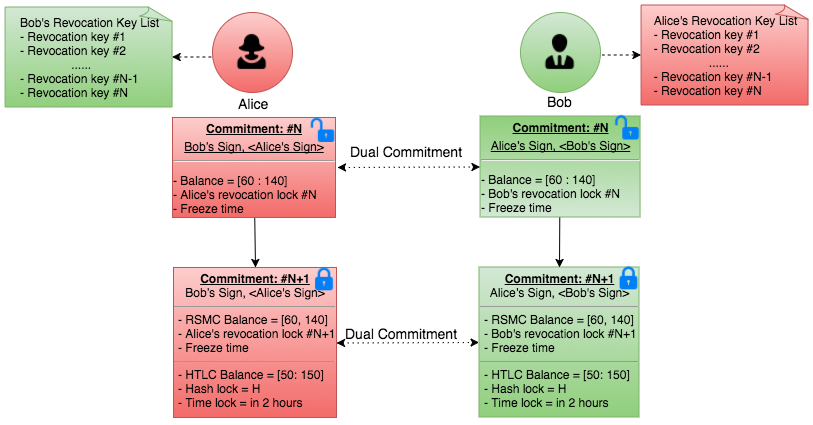
\includegraphics[width=12cm, keepaspectratio]{../images/alice_bob_2.png}
            \caption{Alice-Bob 签署 HTLC 承诺方案}
            \label{fig:htlc_alice_bob_2}
        \end{figure}

    \item 如图 \ref{fig:htlc_bob_carol_2},Bob 再和 Carol 达成编号为 $\#(M+1)$ 的 HTLC 承诺:如果 Carol 能在更短的时间 \textbf{1小时} 内出示暗语 R,使得 hash(R) = H, 那么Bob 向 Carol 支付 10 美元。同时覆盖 $\#(M)$ 的承诺方案。
        \begin{figure}[h!]
            \centering
            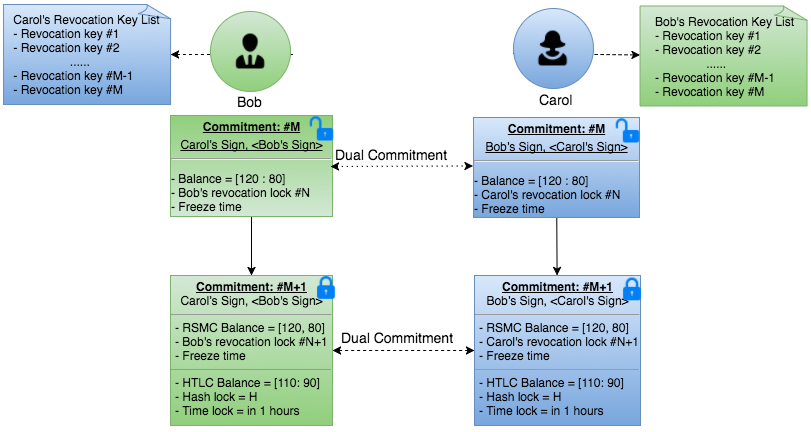
\includegraphics[width=12cm, keepaspectratio]{../images/bob_carol_2.png}
            \caption{Bob-Carol 签署 HTLC 承诺方案}
            \label{fig:htlc_bob_carol_2}
        \end{figure}

    \item 如图 \ref{fig:htlc_bob_carol_3}, 由于 Carol 知道暗语 R 值,在规定的期限T内,可以把R出示给 Bob,获得 Bob 的10美元。之后 Bob 和 Carol 可以再签署一份编号为  RSMC 承诺方案,代替编号为 $\#(M+1)$ 的HTLC 承诺方案。

        \begin{figure}[h!]
            \centering
            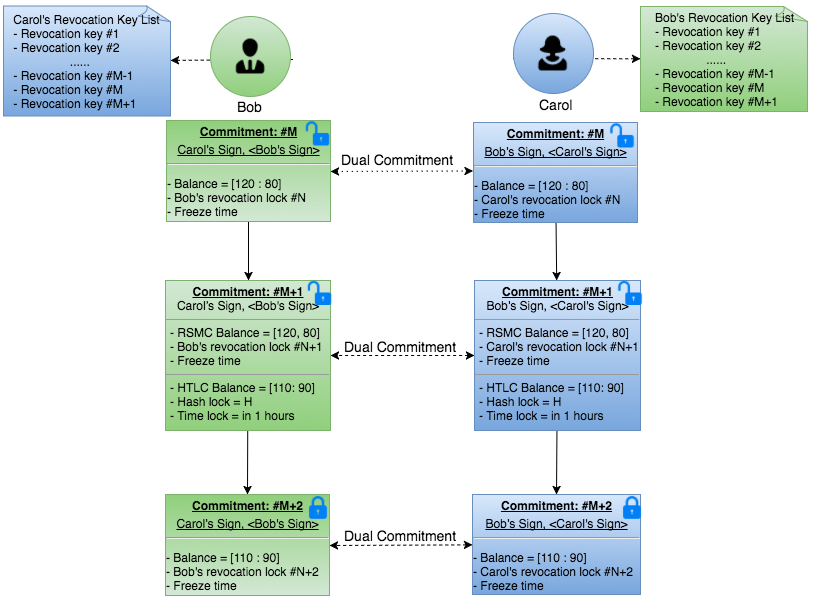
\includegraphics[width=12cm, keepaspectratio]{../images/bob_carol_3.png}
            \caption{Bob 向 Carol 支付 10 美元}
            \label{fig:htlc_bob_carol_3}
        \end{figure}

    \item 如图 \ref{fig:htlc_alice_bob_3},Bob 从 Carol 那里拿到暗语 R 的时候,和 Alice 之间的 HTLC 承诺还没有过期,向 Alice 出示 R 之后,可以获得 10 美元。然后也可以再重新签署一份编号为 $\#(N+2)$ 的 RSMC 承诺,代替编号为 $\#(N+1)$ 的HTLC 承诺方案。
        \begin{figure}[h!]
            \centering
            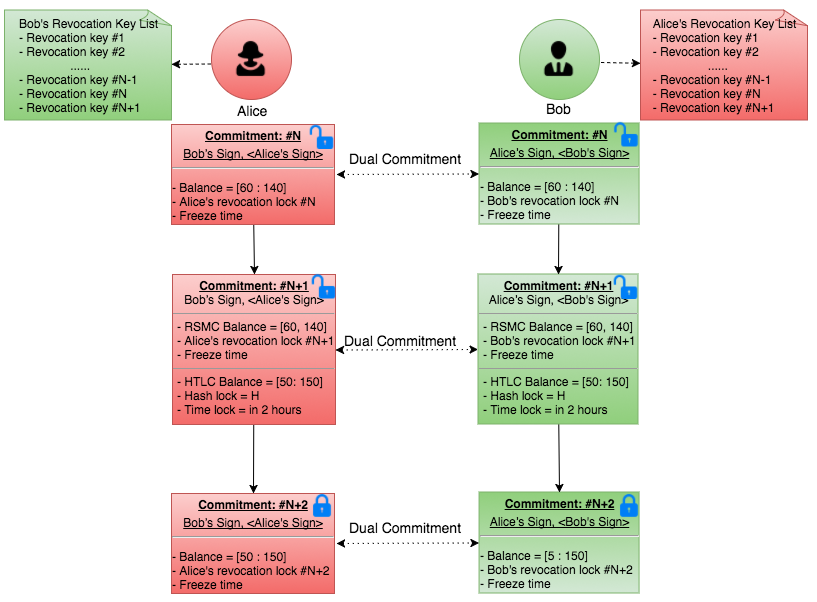
\includegraphics[width=12cm, keepaspectratio]{../images/alice_bob_3.png}
            \caption{Alice 向 Bob 支付 10 美元}
            \label{fig:htlc_alice_bob_3}
        \end{figure}
\end{enumerate}

最终的结果就是:Alice 通过 Bob 向 Carol 支付了 10美元,Bob 作为中间人资产并没有变化。
HTLC 承诺方案可以在两个联通的支付通道上传递交易,这两个支付通道的交易是具有原子性的。

\subsubsection{支付通道内的对手风险}
我们来分析一下,在上一节 \ref{sec:htlc_pay} 的支付过程中对手风险问题,理性的参与者是否自愿地完成支付过程。
我们以 Bob-Carol 的支付过程为例展开分析。

\begin{itemize}
  \item 首先,支付的接收方无法伪造暗语 R 而欺诈对方,因为在规定的时间内破解 Hash 锁是不可能的。

  \item 其次,在双方在达成 $\#(M+1)$ 号HTLC 共同承诺之后,要求双方都撤销编号为 $\#M$ 的承诺方案。
        对于接收者 Carol 来讲,新的承诺方案令其有可能得到 10 美元,不会有任何损失,所以会自愿撤销原承诺方案。
        对于支付方 Bob 方来讲,只有当 Carol 在规定时间内公开暗语 R 的时候才能获得 10 没有,否则就恢复原状。
        所以撤销 $\#M$ 号承诺也没有什么损失。

  \item 再次,双方在达成  $\#(M+1)$ 号 HTLC 共同承诺之后,要求接受者 Carol 在规定时间内公开暗语 R 。
        否则超时之后 HTLC 分配方案失效 Carol 就拿不到 10 美元。

  \item 最后,公开暗语 R 之后,双方可以在一小时的到期之前,建立 $\#(M+2)$ 号长期有效的 RSMC 承诺方案。
        双方要撤销 $\#(M+1)$ 号 HTLC 承诺方案。
        接收方 Carol 无疑会乐意使用新方案代替旧方案。
        对于发送方 Bob 来讲,不配合也没有意义,Carol 依然能够无风险的获得 10 美元。
        因为假如 Bob 不配合,想拖延时间。
        Carol 可以及时提交 $\#(M+1)$ 号 HTLC 承诺方案,兑现属于自己的10美元。
        为了保持支付通道,Bob 也必须自愿的更换新的承诺方案。

\end{itemize}

\subsubsection{支付通道间的对手风险}
下面来分析一下跨支付通道的对手风险问题。
注意到 HTLC 承诺方案是沿着支付路径,从发送方向接收方建立;然后再反方向,从接收方向发送方传递暗语 R,依次完成支付。

对于任何一个中间节点来讲,必须先完成右端的支付才能知道暗语 R,否则无法从左侧的支付通道中获得 10 美元的补偿。
另一方面,由于左侧的 HTLC 超时时间比右侧的长,当他完成右侧的支付并获得暗语 R 之后,有充足的时间在左侧支付通道获得 10 美元。这就保证了两侧支付的原子性。

对于更长的支付路径,HTLC 承诺方案依然有效。
需要注意的是,资金从接收方向发送方传播,每经过一段支付通道,对应的超时时间要增加一个小时,保证资金的发送方有足够的时间向接收到下一个发送方的资金。

进一步推广,所有的支付通道链接在一起构成了\textbf{支付通道网络},其中某一些特定的节点作为中心枢纽,链接其它普通节点。一个节点要向另一个节点支付,只要找到一条联通二者的路径,而且路径上的每一段都都有充足的额度,就可以通过这条路径完成价值转移到过程。

\subsection{支付通道的信任机制}
综上所述,支付通道的本质是以智能合约托管双方的资产,并且通过双方的自治完成债权的清算。
闪电网络设计了一个均衡的二元博弈机制,保证任何一方在自治的过程中不会作弊。
这和中本聪的 POW 共识机制有相似的作用。

具体的来讲,在承诺方案的决策过程中,首先是防御方对承诺方案签名,拥有\textbf{初审权},可以拒绝对防御方不利的条款;
然后进攻方对承诺方案签名,拥有\textbf{复审权},可以放弃对于进攻方不利的方案。二者的权利是对等的。

在承诺方案的执行过程中,进攻方拥有\textbf{主动提交权},有权选择什么时候提交、提交哪一个承诺方案;
防御方拥有\textbf{监督权},有权检查承诺方案的有效性,挑战撤销锁,惩罚进攻方的违约行为;
虚拟银行智能合约拥有\textbf{执行权},公开、公平的按照承诺方案的条款处置双方的资产。
三者的权利是不同的,既互相独立、又互相制约。

\begin{figure}[h!]
    \centering
    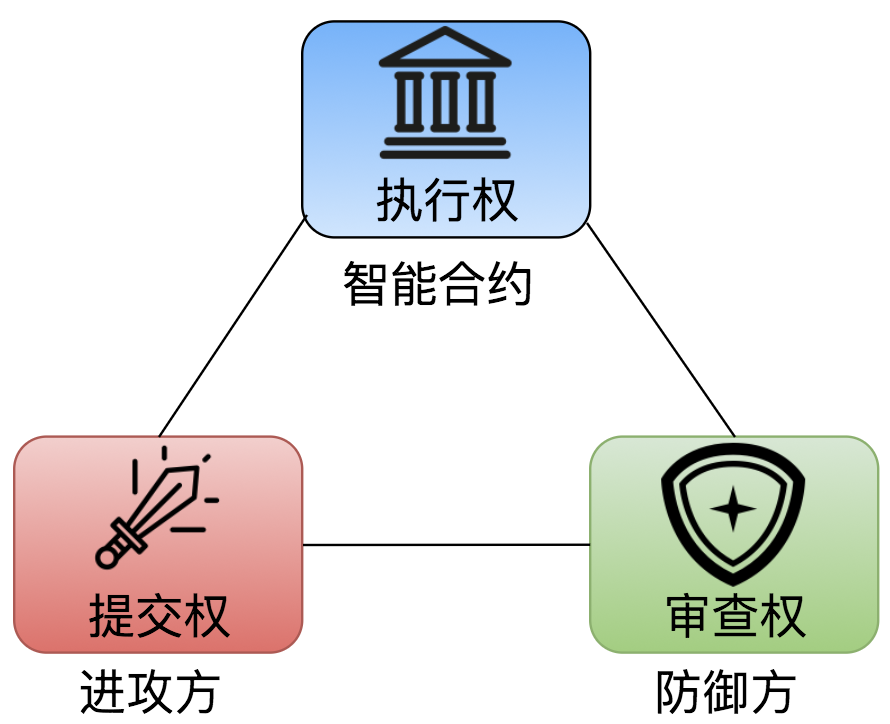
\includegraphics[width=6cm, keepaspectratio]{../images/trias.png}
    \caption{三权分立}
    \label{fig:trias}
\end{figure}

无论是决策阶段、还是执行阶段,虚拟银行的两个用户之间的权利和责任是对等的,谁也无法通过作弊获得不当利益。
这种博弈的纳什均衡点,形成一种内生的信任机制,不需要外部的第三方监管与信用保障。
就像有“一只看不见的手”,自动促使双方必须诚实的遵守共同承诺。

